% PERFORMANCE MEASURE REPORT
% by Marco Giacomin

\section{System Performance Evaluation}

The project specifications require two distinct performance 
measures to judge the quality of the segmentation produced 
by the program:

\begin{enumerate}
    \item Mean average precision (mAP) for ball localization
    \item Mean intersection over union (mIoU) for the class segmentation
\end{enumerate}



\subsection{Intersection over Union (IoU)}

This is the more straightforward of the two measures. 
Given any kind of prediction-truth pairs that represent 
areas (be it a binary mask or a 2d rectangle), the IoU is 
simply the ratio between the area of the intersection of the 
two surfaces and their union.

\begin{figure}[h]
    \centering
    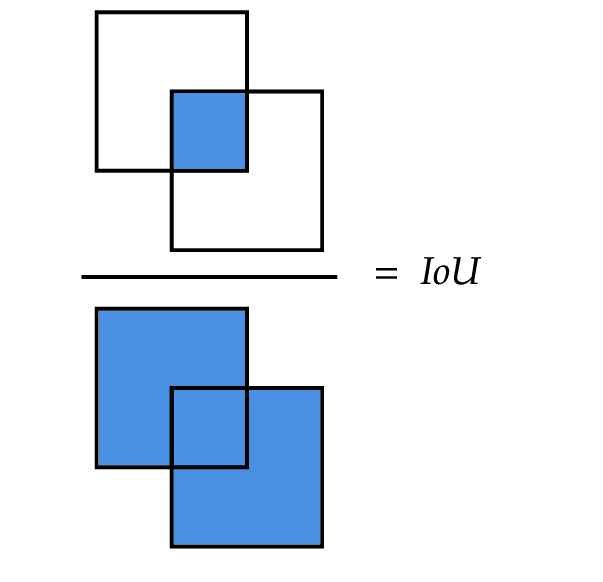
\includegraphics[width=0.4\textwidth]{./imgs/iou.png}
    \caption{Graphical representation of IoU}
\end{figure}

Intuitively, this can be used to represent how well a singular 
prediction in an object detection task fits on the corresponding 
ground truth.
OpenCV provides easy ways to intersect both binary masks and 
\verb|cv::Rect| objects, the first by pixel-wise logical AND 
and the second by a dedicated function.
Union area is instead directly calculated by adding the 
areas of the two surfaces and subtracting the area of 
their intersection.


\subsection{Average precision}

For each ball class for which we make predictions, we are going to 
calculate a metric known as average precision (AP), which is the 
area under the precision-recall curve of the class, per-image, estimated 
using the technique described in the linked article on the project specifications.
For each predicted bounding box, we calculate its maximum IoU with the 
set of ground truths, then we consider it a true positive if the 
value is more than a certain threshold (0.5 in this case). 
We keep a tally of true vs false positives and use it to calculate 
the partial precision and recall values, which we plot in a sparse 
graph (here represented as a \verb|std::map| object).

The area under this graph gives us information on how well the 
localization is performing (1 denotes a perfect classifier, 0 a 
completely wrong one). Since we've build a sparse graph, the 
approximation method PASCAL VOC is used to calculate the 
underlying area: 11 equally spaced points are taken in the 
recall interval (from 0 to 1). For each of those, the corresponding 
precision value is defined as the highest one among all the 
points to the right of it.

\begin{figure}[h]
    \centering
    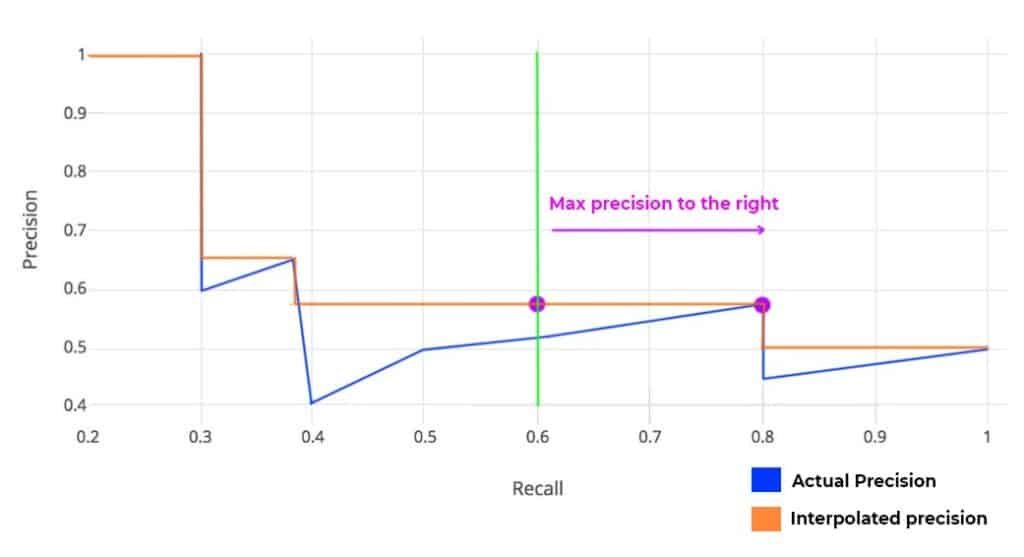
\includegraphics[width=0.4\textwidth]{./imgs/average_precision_graph.jpg}
    \caption{Underlying area estimation of a sparse graph}
\end{figure}

The estimation is the average of the 11 values found this way. The "mean" 
in Mean Average Precision is simply the average of all the AP scores 
calculated for each ball class.

\textbf{Note:} in some clips we might have empty classes (for example, an 
endgame position where all the striped balls have been scored). The 
AP for such cases is defined as 1.


% DO NOT DELETE THIS
\vspace{16cm}
\section{Results}
